%%%%%%%%%%%%%%%%%%%%%%%%%%%%%%%%%%%%%%%%%%%%%%%%%%%%%%%%%%%%%%%%%%%%%%%%%%%%%%%%%%
%%%%  UTA Ph.D. Dissertation Document Generation Using Tex/Latex   %%%%%%%%%%%%%%%%%%%
%%%%%%%%%%%%%%%%%%%%%%%%%%%%%%%%%%%%%%%%%%%%%%%%%%%%%%%%%%%%%%%%%%%%%%%%%%%%%%%%%%
%     Tex/Latex is one of the widely used software to generate many technical and other
%     documents including thesis/dissertations at many universities including UTA.
%
%     The advantage of using Tex/Latex is that with proper style files, most of the
%     front matter required by the university is generated with very little
%     effort (including table of contents, copyright page, list of figures, etc.).
%     All other formatting (margins, fonts, footnote style, equation style,
%     table style, etc.) is built into the style file. With proper style files,
%     it is possible to convert many of the material in any Tex/Latex document
%     so that the generated output fulfills the requirements of an outside publication.
%     Many of the outside publications provide such style files for the conversion.
%
%     The utathesis.zip contains all the sample files that are necessary to generate
%     a typical UTA Ph.D. Dissertation Document including utathesis.sty (contains
%     all the formatting required by UTA Graduate School), graphics.sty, psfig.sty
%     (to include figures that may be in the thesis), amsmath.sty (helpful in generating
%     more complex equations), two typical chapters (which contain equations, figures, and
%     tables, references), two appendices, typical dedication, acknowledgement, abstract,
%     and biographic information files. It is suggested that you unzip utathesis.zip
%     into a new directory so that you can run utaexample.tex contained in
%     the directory to generate a sample output. The utaexample.tex is like a script file
%     which you can modify to suit individual requirements and any minor changes that
%     are required. By commenting out certain portions of the utaexample.tex, it is
%     possible to generate truncated output (just one chapter without front matter, etc.).
%
%     Any Tex/Latex Package including MiKTex (http://www.miktex.org)
%     and Convenience Tex/Latex Editors (http://www.miktex.org/links.html) may be used
%     to generate the Dissertation Document.
%
%     This utaexample.tex file was created by UTA EE Department and uses the
%     bibliography/reference style used by IEEE and adopted by EE Department.
%     The bibliography/reference file acceptable to other departments at UTA are available
%     and must be substituted in the appropriate place.
%
%     Any comments/suggestions  you may have may be sent to prabhu@uta.edu.
%
%%%%%%%%%%%%%%%%%%%%%%%%%%%%%%%%%%%%%%%%%%%%%%%%%%%%%%%%%%%%%%%%%%%%%%%%%%%%%%%%%%

%%%%%%%%%%%%%%%%%%%%%%%%%%%%%%%%%%%%%%%%%%%%%%%%%%%%%%%%%%%%%%%%%%%%%%%%%%%%%%%%%%
%%%%  UTA Ph.D. Dissertation Document Generation Using Tex/Latex   %%%%%%%%%%%%%%%%%%%
%%%%%%%%%%%%%%%%%%%%%%%%%%%%%%%%%%%%%%%%%%%%%%%%%%%%%%%%%%%%%%%%%%%%%%%%%%%%%%%%%%

%%%%%%%%%%%%%%%%%%%%%%%%%%%%%%%%%%%%%%%%%%%%%%%%%%%%%%%%%%%%%%%%%%%%%%%%%%%%%%%%%%
%%%%%%%%%%%%%%%%         all the preamble material            %%%%%%%%%%%%%%%%%%%%
%%%%%%%%%%%%%%%%%%%%%%%%%%%%%%%%%%%%%%%%%%%%%%%%%%%%%%%%%%%%%%%%%%%%%%%%%%%%%%%%%%

% packages
\documentclass[12pt]{report}\usepackage{utathesis,amsmath,amsthm,amssymb,listings,color,graphicx,float,enumitem,algorithm,algpseudocode,oldgerm,mathrsfs,microtype,geometry,latexsym,xpatch,etoolbox,tikz,bm}%,showkeys}
\usepackage[english]{babel}
\usepackage[utf8x]{inputenc}
\usepackage{mdframed}

% for units
\usepackage{siunitx}

% for the vector on ones
\usepackage{bbm}

% to get the units correctly for printing
\usepackage{layouts}

% Sample bibliography materials
% Entries found here: http://ctan.math.utah.edu/ctan/tex-archive/macros/latex/contrib/biblatex/bibtex/bib/biblatex/biblatex-examples.bib
%\usepackage{biblatex}


% A nice way to customize commands, e.g., \C instead of \mathfrak{C} for the set of complex numbers
% Suggestion: name macros specific to document: macros_diss, macros_colloquium, etc.
\input macros_disstemplate.tex

\begin{document}
    % Psfig/TeX 
\def\PsfigVersion{1.10}
\def\setDriver{\DvipsDriver} % \DvipsDriver or \OzTeXDriver
%
% All software, documentation, and related files in this distribution of
% psfig/tex are Copyright 1993 Trevor J. Darrell
%
% Permission is granted for use and non-profit distribution of psfig/tex 
% providing that this notice is clearly maintained. The right to
% distribute any portion of psfig/tex for profit or as part of any commercial
% product is specifically reserved for the author(s) of that portion.
%
% To use with LaTeX, use \documentstyle[psfig,...]{...}
% To use with TeX, use \input psfig.sty
%
% Bugs and improvements to trevor@media.mit.edu.
%
% Thanks to Ned Batchelder, Greg Hager (GDH), J. Daniel Smith (JDS),
% Tom Rokicki (TR), Robert Russell (RR), George V. Reilly (GVR),
% Ken McGlothlen (KHC), Baron Grey (BG), Gerhard Tobermann (GT).
% and all others who have contributed code and comments to this project!
%
% ======================================================================
% Modification History:
%
%  9 Oct 1990   JDS	used more robust bbox reading code from Tom Rokicki
% 29 Mar 1991   JDS	implemented rotation= option
% 25 Jun 1991   RR	if bb specified on cmd line don't check
%			for .ps file.
%  3 Jul 1991	JDS	check if file already read in once
%  4 Sep 1991	JDS	fixed incorrect computation of rotated
%			bounding box
% 25 Sep 1991	GVR	expanded synopsis of \psfig
% 14 Oct 1991	JDS	\fbox code from LaTeX so \psdraft works with TeX
%			changed \typeout to \ps@typeout
% 17 Oct 1991	JDS	added \psscalefirst and \psrotatefirst
% 23 Jun 1993   KHC     ``doclip'' must appear before ``rotate''
% 27 Oct 1993   TJD	removed printing of filename to avoid 
%			underscore problems. changed \frame to \fbox.
%			Added OzTeX support from BG. Added new
%			figure search path code from GT.
%
% ======================================================================
%
% Command synopsis:
%
% \psdraft	draws an outline box, but doesn't include the figure
%		in the DVI file.  Useful for previewing.
%
% \psfull	includes the figure in the DVI file (default).
%
% \psscalefirst width= or height= specifies the size of the figure
% 		before rotation.
% \psrotatefirst (default) width= or height= specifies the size of the
% 		 figure after rotation.  Asymetric figures will
% 		 appear to shrink.
%
% \psfigurepath{dir:dir:...}  sets the path to search for the figure
%
% \psfig
% usage: \psfig{file=, figure=, height=, width=,
%			bbllx=, bblly=, bburx=, bbury=,
%			rheight=, rwidth=, clip=, angle=, silent=}
%
%	"file" is the filename.  If no path name is specified and the
%		file is not found in the current directory,
%		it will be looked for in directory \psfigurepath.
%	"figure" is a synonym for "file".
%	By default, the width and height of the figure are taken from
%		the BoundingBox of the figure.
%	If "width" is specified, the figure is scaled so that it has
%		the specified width.  Its height changes proportionately.
%	If "height" is specified, the figure is scaled so that it has
%		the specified height.  Its width changes proportionately.
%	If both "width" and "height" are specified, the figure is scaled
%		anamorphically.
%	"bbllx", "bblly", "bburx", and "bbury" control the PostScript
%		BoundingBox.  If these four values are specified
%               *before* the "file" option, the PSFIG will not try to
%               open the PostScript file.
%	"rheight" and "rwidth" are the reserved height and width
%		of the figure, i.e., how big TeX actually thinks
%		the figure is.  They default to "width" and "height".
%	The "clip" option ensures that no portion of the figure will
%		appear outside its BoundingBox.  "clip=" is a switch and
%		takes no value, but the `=' must be present.
%	The "angle" option specifies the angle of rotation (degrees, ccw).
%	The "silent" option makes \psfig work silently.
%
% ======================================================================
% check to see if macros already loaded in (maybe some other file says
% "\input psfig") ...
\ifx\undefined\psfig\else\endinput\fi
%
% from a suggestion by eijkhout@csrd.uiuc.edu to allow
% loading as a style file. Changed to avoid problems
% with amstex per suggestion by jbence@math.ucla.edu

\let\LaTeXAtSign=\@
\let\@=\relax
\edef\psfigRestoreAt{\catcode`\@=\number\catcode`@\relax}
%\edef\psfigRestoreAt{\catcode`@=\number\catcode`@\relax}
\catcode`\@=11\relax
\newwrite\@unused
\def\ps@typeout#1{{\let\protect\string\immediate\write\@unused{#1}}}

\def\DvipsDriver{
	\ps@typeout{psfig/tex \PsfigVersion -dvips}
\def\PsfigSpecials{\DvipsSpecials} 	\def\ps@dir{/}
\def\ps@predir{} }
\def\OzTeXDriver{
	\ps@typeout{psfig/tex \PsfigVersion -oztex}
	\def\PsfigSpecials{\OzTeXSpecials}
	\def\ps@dir{:}
	\def\ps@predir{:}
	\catcode`\^^J=5
}

%% Here's how you define your figure path.  Should be set up with null
%% default and a user useable definition.

\def\figurepath{./:}
\def\psfigurepath#1{\edef\figurepath{#1:}}

%%% inserted for Searching Unixpaths
%%% (the path must end with :)
%%% (call: \DoPaths\figurepath )
%%%------------------------------------------------------
\def\DoPaths#1{\expandafter\EachPath#1\stoplist}
%
\def\leer{}
\def\EachPath#1:#2\stoplist{% #1 part of the list (delimiter :)
  \ExistsFile{#1}{\SearchedFile}
  \ifx#2\leer
  \else
    \expandafter\EachPath#2\stoplist
  \fi}
%
% exists the file (does not work for directories!)
%
\def\ps@dir{/}
\def\ExistsFile#1#2{%
   \openin1=\ps@predir#1\ps@dir#2
   \ifeof1
       \closein1
       %\ps@typeout{...not: \ps@predir#1\ps@dir#2}
   \else
       \closein1
       %\ps@typeout{...in:  \ps@predir#1\ps@dir#2}
        \ifx\ps@founddir\leer
          %\ps@typeout{set founddir #1}
           \edef\ps@founddir{#1}
        \fi
   \fi}
%------------------------------------------------------
%
% Get dir in path or error
%
\def\get@dir#1{%
  \def\ps@founddir{}
  \def\SearchedFile{#1}
  \DoPaths\figurepath
%  \fi
}
%------------------------------------------------------
%%% END of Searching Unixpaths


%
% @psdo control structure -- similar to Latex @for.
% I redefined these with different names so that psfig can
% be used with TeX as well as LaTeX, and so that it will not 
% be vunerable to future changes in LaTeX's internal
% control structure,
%
\def\@nnil{\@nil}
\def\@empty{}
\def\@psdonoop#1\@@#2#3{}
\def\@psdo#1:=#2\do#3{\edef\@psdotmp{#2}\ifx\@psdotmp\@empty \else
    \expandafter\@psdoloop#2,\@nil,\@nil\@@#1{#3}\fi}
\def\@psdoloop#1,#2,#3\@@#4#5{\def#4{#1}\ifx #4\@nnil \else
       #5\def#4{#2}\ifx #4\@nnil \else#5\@ipsdoloop #3\@@#4{#5}\fi\fi}
\def\@ipsdoloop#1,#2\@@#3#4{\def#3{#1}\ifx #3\@nnil 
       \let\@nextwhile=\@psdonoop \else
      #4\relax\let\@nextwhile=\@ipsdoloop\fi\@nextwhile#2\@@#3{#4}}
\def\@tpsdo#1:=#2\do#3{\xdef\@psdotmp{#2}\ifx\@psdotmp\@empty \else
    \@tpsdoloop#2\@nil\@nil\@@#1{#3}\fi}
\def\@tpsdoloop#1#2\@@#3#4{\def#3{#1}\ifx #3\@nnil 
       \let\@nextwhile=\@psdonoop \else
      #4\relax\let\@nextwhile=\@tpsdoloop\fi\@nextwhile#2\@@#3{#4}}
% 
% \fbox is defined in latex.tex; so if \fbox is undefined, assume that
% we are not in LaTeX.
% Perhaps this could be done better???
\ifx\undefined\fbox
% \fbox code from modified slightly from LaTeX
\newdimen\fboxrule
\newdimen\fboxsep
\newdimen\ps@tempdima
\newbox\ps@tempboxa
\fboxsep = 3pt
\fboxrule = .4pt
\long\def\fbox#1{\leavevmode\setbox\ps@tempboxa\hbox{#1}\ps@tempdima\fboxrule
    \advance\ps@tempdima \fboxsep \advance\ps@tempdima \dp\ps@tempboxa
   \hbox{\lower \ps@tempdima\hbox
  {\vbox{\hrule height \fboxrule
          \hbox{\vrule width \fboxrule \hskip\fboxsep
          \vbox{\vskip\fboxsep \box\ps@tempboxa\vskip\fboxsep}\hskip 
                 \fboxsep\vrule width \fboxrule}
                 \hrule height \fboxrule}}}}
\fi
%
%%%%%%%%%%%%%%%%%%%%%%%%%%%%%%%%%%%%%%%%%%%%%%%%%%%%%%%%%%%%%%%%%%%
% file reading stuff from epsf.tex
%   EPSF.TEX macro file:
%   Written by Tomas Rokicki of Radical Eye Software, 29 Mar 1989.
%   Revised by Don Knuth, 3 Jan 1990.
%   Revised by Tomas Rokicki to accept bounding boxes with no
%      space after the colon, 18 Jul 1990.
%   Portions modified/removed for use in PSFIG package by
%      J. Daniel Smith, 9 October 1990.
%
\newread\ps@stream
\newif\ifnot@eof       % continue looking for the bounding box?
\newif\if@noisy        % report what you're making?
\newif\if@atend        % %%BoundingBox: has (at end) specification
\newif\if@psfile       % does this look like a PostScript file?
%
% PostScript files should start with `%!'
%
{\catcode`\%=12\global\gdef\epsf@start{%!}}
\def\epsf@PS{PS}
%
\def\epsf@getbb#1{%
%
%   The first thing we need to do is to open the
%   PostScript file, if possible.
%
\openin\ps@stream=\ps@predir#1
\ifeof\ps@stream\ps@typeout{Error, File #1 not found}\else
%
%   Okay, we got it. Now we'll scan lines until we find one that doesn't
%   start with %. We're looking for the bounding box comment.
%
   {\not@eoftrue \chardef\other=12
    \def\do##1{\catcode`##1=\other}\dospecials \catcode`\ =10
    \loop
       \if@psfile
	  \read\ps@stream to \epsf@fileline
       \else{
	  \obeyspaces
          \read\ps@stream to \epsf@tmp\global\let\epsf@fileline\epsf@tmp}
       \fi
       \ifeof\ps@stream\not@eoffalse\else
%
%   Check the first line for `%!'.  Issue a warning message if its not
%   there, since the file might not be a PostScript file.
%
       \if@psfile\else
       \expandafter\epsf@test\epsf@fileline:. \\%
       \fi
%
%   We check to see if the first character is a % sign;
%   if so, we look further and stop only if the line begins with
%   `%%BoundingBox:' and the `(atend)' specification was not found.
%   That is, the only way to stop is when the end of file is reached,
%   or a `%%BoundingBox: llx lly urx ury' line is found.
%
          \expandafter\epsf@aux\epsf@fileline:. \\%
       \fi
   \ifnot@eof\repeat
   }\closein\ps@stream\fi}%
%
% This tests if the file we are reading looks like a PostScript file.
%
\long\def\epsf@test#1#2#3:#4\\{\def\epsf@testit{#1#2}
			\ifx\epsf@testit\epsf@start\else
\ps@typeout{Warning! File does not start with `\epsf@start'.  It may not be a PostScript file.}
			\fi
			\@psfiletrue} % don't test after 1st line
%
%   We still need to define the tricky \epsf@aux macro. This requires
%   a couple of magic constants for comparison purposes.
%
{\catcode`\%=12\global\let\epsf@percent=%\global\def\epsf@bblit{%BoundingBox}}
%
%
%   So we're ready to check for `%BoundingBox:' and to grab the
%   values if they are found.  We continue searching if `(at end)'
%   was found after the `%BoundingBox:'.
%
\long\def\epsf@aux#1#2:#3\\{\ifx#1\epsf@percent
   \def\epsf@testit{#2}\ifx\epsf@testit\epsf@bblit
	\@atendfalse
        \epsf@atend #3 . \\%
	\if@atend	
	   \if@verbose{
		\ps@typeout{psfig: found `(atend)'; continuing search}
	   }\fi
        \else
        \epsf@grab #3 . . . \\%
        \not@eoffalse
        \global\no@bbfalse
        \fi
   \fi\fi}%
%
%   Here we grab the values and stuff them in the appropriate definitions.
%
\def\epsf@grab #1 #2 #3 #4 #5\\{%
   \global\def\epsf@llx{#1}\ifx\epsf@llx\empty
      \epsf@grab #2 #3 #4 #5 .\\\else
   \global\def\epsf@lly{#2}%
   \global\def\epsf@urx{#3}\global\def\epsf@ury{#4}\fi}%
%
% Determine if the stuff following the %%BoundingBox is `(atend)'
% J. Daniel Smith.  Copied from \epsf@grab above.
%
\def\epsf@atendlit{(atend)} 
\def\epsf@atend #1 #2 #3\\{%
   \def\epsf@tmp{#1}\ifx\epsf@tmp\empty
      \epsf@atend #2 #3 .\\\else
   \ifx\epsf@tmp\epsf@atendlit\@atendtrue\fi\fi}


% End of file reading stuff from epsf.tex
%%%%%%%%%%%%%%%%%%%%%%%%%%%%%%%%%%%%%%%%%%%%%%%%%%%%%%%%%%%%%%%%%%%

%%%%%%%%%%%%%%%%%%%%%%%%%%%%%%%%%%%%%%%%%%%%%%%%%%%%%%%%%%%%%%%%%%%
% trigonometry stuff from "trig.tex"
\chardef\psletter = 11 % won't conflict with \begin{letter} now...
\chardef\other = 12

\newif \ifdebug %%% turn me on to see TeX hard at work ...
\newif\ifc@mpute %%% don't need to compute some values
\c@mputetrue % but assume that we do

\let\then = \relax
\def\r@dian{pt }
\let\r@dians = \r@dian
\let\dimensionless@nit = \r@dian
\let\dimensionless@nits = \dimensionless@nit
\def\internal@nit{sp }
\let\internal@nits = \internal@nit
\newif\ifstillc@nverging
\def \Mess@ge #1{\ifdebug \then \message {#1} \fi}

{ %%% Things that need abnormal catcodes %%%
	\catcode `\@ = \psletter
	\gdef \nodimen {\expandafter \n@dimen \the \dimen}
	\gdef \term #1 #2 #3%
	       {\edef \t@ {\the #1}%%% freeze parameter 1 (count, by value)
		\edef \t@@ {\expandafter \n@dimen \the #2\r@dian}%
				   %%% freeze parameter 2 (dimen, by value)
		\t@rm {\t@} {\t@@} {#3}%
	       }
	\gdef \t@rm #1 #2 #3%
	       {{%
		\count 0 = 0
		\dimen 0 = 1 \dimensionless@nit
		\dimen 2 = #2\relax
		\Mess@ge {Calculating term #1 of \nodimen 2}%
		\loop
		\ifnum	\count 0 < #1
		\then	\advance \count 0 by 1
			\Mess@ge {Iteration \the \count 0 \space}%
			\Multiply \dimen 0 by {\dimen 2}%
			\Mess@ge {After multiplication, term = \nodimen 0}%
			\Divide \dimen 0 by {\count 0}%
			\Mess@ge {After division, term = \nodimen 0}%
		\repeat
		\Mess@ge {Final value for term #1 of 
				\nodimen 2 \space is \nodimen 0}%
		\xdef \Term {#3 = \nodimen 0 \r@dians}%
		\aftergroup \Term
	       }}
	\catcode `\p = \other
	\catcode `\t = \other
	\gdef \n@dimen #1pt{#1} %%% throw away the ``pt''
}

\def \Divide #1by #2{\divide #1 by #2} %%% just a synonym

\def \Multiply #1by #2%%% allows division of a dimen by a dimen
       {{%%% should really freeze parameter 2 (dimen, passed by value)
	\count 0 = #1\relax
	\count 2 = #2\relax
	\count 4 = 65536
	\Mess@ge {Before scaling, count 0 = \the \count 0 \space and
			count 2 = \the \count 2}%
	\ifnum	\count 0 > 32767 %%% do our best to avoid overflow
	\then	\divide \count 0 by 4
		\divide \count 4 by 4
	\else	\ifnum	\count 0 < -32767
		\then	\divide \count 0 by 4
			\divide \count 4 by 4
		\else
		\fi
	\fi
	\ifnum	\count 2 > 32767 %%% while retaining reasonable accuracy
	\then	\divide \count 2 by 4
		\divide \count 4 by 4
	\else	\ifnum	\count 2 < -32767
		\then	\divide \count 2 by 4
			\divide \count 4 by 4
		\else
		\fi
	\fi
	\multiply \count 0 by \count 2
	\divide \count 0 by \count 4
	\xdef \product {#1 = \the \count 0 \internal@nits}%
	\aftergroup \product
       }}

\def\r@duce{\ifdim\dimen0 > 90\r@dian \then   % sin(x+90) = sin(180-x)
		\multiply\dimen0 by -1
		\advance\dimen0 by 180\r@dian
		\r@duce
	    \else \ifdim\dimen0 < -90\r@dian \then  % sin(-x) = sin(360+x)
		\advance\dimen0 by 360\r@dian
		\r@duce
		\fi
	    \fi}

\def\Sine#1%
       {{%
	\dimen 0 = #1 \r@dian
	\r@duce
	\ifdim\dimen0 = -90\r@dian \then
	   \dimen4 = -1\r@dian
	   \c@mputefalse
	\fi
	\ifdim\dimen0 = 90\r@dian \then
	   \dimen4 = 1\r@dian
	   \c@mputefalse
	\fi
	\ifdim\dimen0 = 0\r@dian \then
	   \dimen4 = 0\r@dian
	   \c@mputefalse
	\fi
%
	\ifc@mpute \then
        	% convert degrees to radians
		\divide\dimen0 by 180
		\dimen0=3.141592654\dimen0
%
		\dimen 2 = 3.1415926535897963\r@dian %%% a well-known constant
		\divide\dimen 2 by 2 %%% we only deal with -pi/2 : pi/2
		\Mess@ge {Sin: calculating Sin of \nodimen 0}%
		\count 0 = 1 %%% see power-series expansion for sine
		\dimen 2 = 1 \r@dian %%% ditto
		\dimen 4 = 0 \r@dian %%% ditto
		\loop
			\ifnum	\dimen 2 = 0 %%% then we've done
			\then	\stillc@nvergingfalse 
			\else	\stillc@nvergingtrue
			\fi
			\ifstillc@nverging %%% then calculate next term
			\then	\term {\count 0} {\dimen 0} {\dimen 2}%
				\advance \count 0 by 2
				\count 2 = \count 0
				\divide \count 2 by 2
				\ifodd	\count 2 %%% signs alternate
				\then	\advance \dimen 4 by \dimen 2
				\else	\advance \dimen 4 by -\dimen 2
				\fi
		\repeat
	\fi		
			\xdef \sine {\nodimen 4}%
       }}

% Now the Cosine can be calculated easily by calling \Sine
\def\Cosine#1{\ifx\sine\UnDefined\edef\Savesine{\relax}\else
		             \edef\Savesine{\sine}\fi
	{\dimen0=#1\r@dian\advance\dimen0 by 90\r@dian
	 \Sine{\nodimen 0}
	 \xdef\cosine{\sine}
	 \xdef\sine{\Savesine}}}	      
% end of trig stuff
%%%%%%%%%%%%%%%%%%%%%%%%%%%%%%%%%%%%%%%%%%%%%%%%%%%%%%%%%%%%%%%%%%%%

\def\psdraft{
	\def\@psdraft{0}
	%\ps@typeout{draft level now is \@psdraft \space . }
}
\def\psfull{
	\def\@psdraft{100}
	%\ps@typeout{draft level now is \@psdraft \space . }
}

\psfull

\newif\if@scalefirst
\def\psscalefirst{\@scalefirsttrue}
\def\psrotatefirst{\@scalefirstfalse}
\psrotatefirst

\newif\if@draftbox
\def\psnodraftbox{
	\@draftboxfalse
}
\def\psdraftbox{
	\@draftboxtrue
}
\@draftboxtrue

\newif\if@prologfile
\newif\if@postlogfile
\def\pssilent{
	\@noisyfalse
}
\def\psnoisy{
	\@noisytrue
}
\psnoisy
%%% These are for the option list.
%%% A specification of the form a = b maps to calling \@p@@sa{b}
\newif\if@bbllx
\newif\if@bblly
\newif\if@bburx
\newif\if@bbury
\newif\if@height
\newif\if@width
\newif\if@rheight
\newif\if@rwidth
\newif\if@angle
\newif\if@clip
\newif\if@verbose
\def\@p@@sclip#1{\@cliptrue}
%
%
\newif\if@decmpr
%
\def\@p@@sfigure#1{\def\@p@sfile{null}\def\@p@sbbfile{null}\@decmprfalse
   % look directly for file (e.g. absolute path)
   \openin1=\ps@predir#1
   \ifeof1
	\closein1
	% failed, search directories for file
	\get@dir{#1}
	\ifx\ps@founddir\leer
		% failed, search directly for file.bb
		\openin1=\ps@predir#1.bb
		\ifeof1
			\closein1
			% failed, search directories for file.bb
			\get@dir{#1.bb}
			\ifx\ps@founddir\leer
				% failed, lose.
				\ps@typeout{Can't find #1 in \figurepath}
			\else
				% found file.bb in search dir
				\@decmprtrue
				\def\@p@sfile{\ps@founddir\ps@dir#1}
				\def\@p@sbbfile{\ps@founddir\ps@dir#1.bb}
			\fi
		\else
			\closein1
			%found file.bb directly
			\@decmprtrue
			\def\@p@sfile{#1}
			\def\@p@sbbfile{#1.bb}
		\fi
	\else
		% found file in search dir
		\def\@p@sfile{\ps@founddir\ps@dir#1}
		\def\@p@sbbfile{\ps@founddir\ps@dir#1}
	\fi
   \else
	% found file directly
	\closein1
	\def\@p@sfile{#1}
	\def\@p@sbbfile{#1}
   \fi
}
%
%
%
\def\@p@@sfile#1{\@p@@sfigure{#1}}
%
\def\@p@@sbbllx#1{
		%\ps@typeout{bbllx is #1}
		\@bbllxtrue
		\dimen100=#1
		\edef\@p@sbbllx{\number\dimen100}
}
\def\@p@@sbblly#1{
		%\ps@typeout{bblly is #1}
		\@bbllytrue
		\dimen100=#1
		\edef\@p@sbblly{\number\dimen100}
}
\def\@p@@sbburx#1{
		%\ps@typeout{bburx is #1}
		\@bburxtrue
		\dimen100=#1
		\edef\@p@sbburx{\number\dimen100}
}
\def\@p@@sbbury#1{
		%\ps@typeout{bbury is #1}
		\@bburytrue
		\dimen100=#1
		\edef\@p@sbbury{\number\dimen100}
}
\def\@p@@sheight#1{
		\@heighttrue
		\dimen100=#1
   		\edef\@p@sheight{\number\dimen100}
		%\ps@typeout{Height is \@p@sheight}
}
\def\@p@@swidth#1{
		%\ps@typeout{Width is #1}
		\@widthtrue
		\dimen100=#1
		\edef\@p@swidth{\number\dimen100}
}
\def\@p@@srheight#1{
		%\ps@typeout{Reserved height is #1}
		\@rheighttrue
		\dimen100=#1
		\edef\@p@srheight{\number\dimen100}
}
\def\@p@@srwidth#1{
		%\ps@typeout{Reserved width is #1}
		\@rwidthtrue
		\dimen100=#1
		\edef\@p@srwidth{\number\dimen100}
}
\def\@p@@sangle#1{
		%\ps@typeout{Rotation is #1}
		\@angletrue
%		\dimen100=#1
		\edef\@p@sangle{#1} %\number\dimen100}
}
\def\@p@@ssilent#1{ 
		\@verbosefalse
}
\def\@p@@sprolog#1{\@prologfiletrue\def\@prologfileval{#1}}
\def\@p@@spostlog#1{\@postlogfiletrue\def\@postlogfileval{#1}}
\def\@cs@name#1{\csname #1\endcsname}
\def\@setparms#1=#2,{\@cs@name{@p@@s#1}{#2}}
%
% initialize the defaults (size the size of the figure)
%
\def\ps@init@parms{
		\@bbllxfalse \@bbllyfalse
		\@bburxfalse \@bburyfalse
		\@heightfalse \@widthfalse
		\@rheightfalse \@rwidthfalse
		\def\@p@sbbllx{}\def\@p@sbblly{}
		\def\@p@sbburx{}\def\@p@sbbury{}
		\def\@p@sheight{}\def\@p@swidth{}
		\def\@p@srheight{}\def\@p@srwidth{}
		\def\@p@sangle{0}
		\def\@p@sfile{} \def\@p@sbbfile{}
		\def\@p@scost{10}
		\def\@sc{}
		\@prologfilefalse
		\@postlogfilefalse
		\@clipfalse
		\if@noisy
			\@verbosetrue
		\else
			\@verbosefalse
		\fi
}
%
% Go through the options setting things up.
%
\def\parse@ps@parms#1{
	 	\@psdo\@psfiga:=#1\do
		   {\expandafter\@setparms\@psfiga,}}
%
% Compute bb height and width
%
\newif\ifno@bb
\def\bb@missing{
	\if@verbose{
		\ps@typeout{psfig: searching \@p@sbbfile \space  for bounding box}
	}\fi
	\no@bbtrue
	\epsf@getbb{\@p@sbbfile}
        \ifno@bb \else \bb@cull\epsf@llx\epsf@lly\epsf@urx\epsf@ury\fi
}	
\def\bb@cull#1#2#3#4{
	\dimen100=#1 bp\edef\@p@sbbllx{\number\dimen100}
	\dimen100=#2 bp\edef\@p@sbblly{\number\dimen100}
	\dimen100=#3 bp\edef\@p@sbburx{\number\dimen100}
	\dimen100=#4 bp\edef\@p@sbbury{\number\dimen100}
	\no@bbfalse
}
% rotate point (#1,#2) about (0,0).
% The sine and cosine of the angle are already stored in \sine and
% \cosine.  The result is placed in (\p@intvaluex, \p@intvaluey).
\newdimen\p@intvaluex
\newdimen\p@intvaluey
\def\rotate@#1#2{{\dimen0=#1 sp\dimen1=#2 sp
%            	calculate x' = x \cos\theta - y \sin\theta
		  \global\p@intvaluex=\cosine\dimen0
		  \dimen3=\sine\dimen1
		  \global\advance\p@intvaluex by -\dimen3
% 		calculate y' = x \sin\theta + y \cos\theta
		  \global\p@intvaluey=\sine\dimen0
		  \dimen3=\cosine\dimen1
		  \global\advance\p@intvaluey by \dimen3
		  }}
\def\compute@bb{
		\no@bbfalse
		\if@bbllx \else \no@bbtrue \fi
		\if@bblly \else \no@bbtrue \fi
		\if@bburx \else \no@bbtrue \fi
		\if@bbury \else \no@bbtrue \fi
		\ifno@bb \bb@missing \fi
		\ifno@bb \ps@typeout{FATAL ERROR: no bb supplied or found}
			\no-bb-error
		\fi
		%
%\ps@typeout{BB: \@p@sbbllx, \@p@sbblly, \@p@sbburx, \@p@sbbury} 
%
% store height/width of original (unrotated) bounding box
		\count203=\@p@sbburx
		\count204=\@p@sbbury
		\advance\count203 by -\@p@sbbllx
		\advance\count204 by -\@p@sbblly
		\edef\ps@bbw{\number\count203}
		\edef\ps@bbh{\number\count204}
		%\ps@typeout{ psbbh = \ps@bbh, psbbw = \ps@bbw }
		\if@angle 
			\Sine{\@p@sangle}\Cosine{\@p@sangle}
	        	{\dimen100=\maxdimen\xdef\r@p@sbbllx{\number\dimen100}
					    \xdef\r@p@sbblly{\number\dimen100}
			                    \xdef\r@p@sbburx{-\number\dimen100}
					    \xdef\r@p@sbbury{-\number\dimen100}}
%
% Need to rotate all four points and take the X-Y extremes of the new
% points as the new bounding box.
                        \def\minmaxtest{
			   \ifnum\number\p@intvaluex<\r@p@sbbllx
			      \xdef\r@p@sbbllx{\number\p@intvaluex}\fi
			   \ifnum\number\p@intvaluex>\r@p@sbburx
			      \xdef\r@p@sbburx{\number\p@intvaluex}\fi
			   \ifnum\number\p@intvaluey<\r@p@sbblly
			      \xdef\r@p@sbblly{\number\p@intvaluey}\fi
			   \ifnum\number\p@intvaluey>\r@p@sbbury
			      \xdef\r@p@sbbury{\number\p@intvaluey}\fi
			   }
%			lower left
			\rotate@{\@p@sbbllx}{\@p@sbblly}
			\minmaxtest
%			upper left
			\rotate@{\@p@sbbllx}{\@p@sbbury}
			\minmaxtest
%			lower right
			\rotate@{\@p@sbburx}{\@p@sbblly}
			\minmaxtest
%			upper right
			\rotate@{\@p@sbburx}{\@p@sbbury}
			\minmaxtest
			\edef\@p@sbbllx{\r@p@sbbllx}\edef\@p@sbblly{\r@p@sbblly}
			\edef\@p@sbburx{\r@p@sbburx}\edef\@p@sbbury{\r@p@sbbury}
%\ps@typeout{rotated BB: \r@p@sbbllx, \r@p@sbblly, \r@p@sbburx, \r@p@sbbury}
		\fi
		\count203=\@p@sbburx
		\count204=\@p@sbbury
		\advance\count203 by -\@p@sbbllx
		\advance\count204 by -\@p@sbblly
		\edef\@bbw{\number\count203}
		\edef\@bbh{\number\count204}
		%\ps@typeout{ bbh = \@bbh, bbw = \@bbw }
}
%
% \in@hundreds performs #1 * (#2 / #3) correct to the hundreds,
%	then leaves the result in @result
%
\def\in@hundreds#1#2#3{\count240=#2 \count241=#3
		     \count100=\count240	% 100 is first digit #2/#3
		     \divide\count100 by \count241
		     \count101=\count100
		     \multiply\count101 by \count241
		     \advance\count240 by -\count101
		     \multiply\count240 by 10
		     \count101=\count240	%101 is second digit of #2/#3
		     \divide\count101 by \count241
		     \count102=\count101
		     \multiply\count102 by \count241
		     \advance\count240 by -\count102
		     \multiply\count240 by 10
		     \count102=\count240	% 102 is the third digit
		     \divide\count102 by \count241
		     \count200=#1\count205=0
		     \count201=\count200
			\multiply\count201 by \count100
		 	\advance\count205 by \count201
		     \count201=\count200
			\divide\count201 by 10
			\multiply\count201 by \count101
			\advance\count205 by \count201
			%
		     \count201=\count200
			\divide\count201 by 100
			\multiply\count201 by \count102
			\advance\count205 by \count201
			%
		     \edef\@result{\number\count205}
}
\def\compute@wfromh{
		% computing : width = height * (bbw / bbh)
		\in@hundreds{\@p@sheight}{\@bbw}{\@bbh}
		%\ps@typeout{ \@p@sheight * \@bbw / \@bbh, = \@result }
		\edef\@p@swidth{\@result}
		%\ps@typeout{w from h: width is \@p@swidth}
}
\def\compute@hfromw{
		% computing : height = width * (bbh / bbw)
	        \in@hundreds{\@p@swidth}{\@bbh}{\@bbw}
		%\ps@typeout{ \@p@swidth * \@bbh / \@bbw = \@result }
		\edef\@p@sheight{\@result}
		%\ps@typeout{h from w : height is \@p@sheight}
}
\def\compute@handw{
		\if@height 
			\if@width
			\else
				\compute@wfromh
			\fi
		\else 
			\if@width
				\compute@hfromw
			\else
				\edef\@p@sheight{\@bbh}
				\edef\@p@swidth{\@bbw}
			\fi
		\fi
}
\def\compute@resv{
		\if@rheight \else \edef\@p@srheight{\@p@sheight} \fi
		\if@rwidth \else \edef\@p@srwidth{\@p@swidth} \fi
		%\ps@typeout{rheight = \@p@srheight, rwidth = \@p@srwidth}
}
%		
% Compute any missing values
\def\compute@sizes{
	\compute@bb
	\if@scalefirst\if@angle
% at this point the bounding box has been adjsuted correctly for
% rotation.  PSFIG does all of its scaling using \@bbh and \@bbw.  If
% a width= or height= was specified along with \psscalefirst, then the
% width=/height= value needs to be adjusted to match the new (rotated)
% bounding box size (specifed in \@bbw and \@bbh).
%    \ps@bbw       width=
%    -------  =  ---------- 
%    \@bbw       new width=
% so `new width=' = (width= * \@bbw) / \ps@bbw; where \ps@bbw is the
% width of the original (unrotated) bounding box.
	\if@width
	   \in@hundreds{\@p@swidth}{\@bbw}{\ps@bbw}
	   \edef\@p@swidth{\@result}
	\fi
	\if@height
	   \in@hundreds{\@p@sheight}{\@bbh}{\ps@bbh}
	   \edef\@p@sheight{\@result}
	\fi
	\fi\fi
	\compute@handw
	\compute@resv}
%
%
%
\def\OzTeXSpecials{
	\special{empty.ps /@isp {true} def}
	\special{empty.ps \@p@swidth \space \@p@sheight \space
			\@p@sbbllx \space \@p@sbblly \space
			\@p@sbburx \space \@p@sbbury \space
			startTexFig \space }
	\if@clip{
		\if@verbose{
			\ps@typeout{(clip)}
		}\fi
		\special{empty.ps doclip \space }
	}\fi
	\if@angle{
		\if@verbose{
			\ps@typeout{(rotate)}
		}\fi
		\special {empty.ps \@p@sangle \space rotate \space} 
	}\fi
	\if@prologfile
	    \special{\@prologfileval \space } \fi
	\if@decmpr{
		\if@verbose{
			\ps@typeout{psfig: Compression not available
			in OzTeX version \space }
		}\fi
	}\else{
		\if@verbose{
			\ps@typeout{psfig: including \@p@sfile \space }
		}\fi
		\special{epsf=\@p@sfile \space }
	}\fi
	\if@postlogfile
	    \special{\@postlogfileval \space } \fi
	\special{empty.ps /@isp {false} def}
}
\def\DvipsSpecials{
	%
	\special{ps::[begin] 	\@p@swidth \space \@p@sheight \space
			\@p@sbbllx \space \@p@sbblly \space
			\@p@sbburx \space \@p@sbbury \space
			startTexFig \space }
	\if@clip{
		\if@verbose{
			\ps@typeout{(clip)}
		}\fi
		\special{ps:: doclip \space }
	}\fi
	\if@angle
		\if@verbose{
			\ps@typeout{(clip)}
		}\fi
		\special {ps:: \@p@sangle \space rotate \space} 
	\fi
	\if@prologfile
	    \special{ps: plotfile \@prologfileval \space } \fi
	\if@decmpr{
		\if@verbose{
			\ps@typeout{psfig: including \@p@sfile.Z \space }
		}\fi
		\special{ps: plotfile "`zcat \@p@sfile.Z" \space }
	}\else{
		\if@verbose{
			\ps@typeout{psfig: including \@p@sfile \space }
		}\fi
		\special{ps: plotfile \@p@sfile \space }
	}\fi
	\if@postlogfile
	    \special{ps: plotfile \@postlogfileval \space } \fi
	\special{ps::[end] endTexFig \space }
}
%
% \psfig
% usage : \psfig{file=, height=, width=, bbllx=, bblly=, bburx=, bbury=,
%			rheight=, rwidth=, clip=}
%
% "clip=" is a switch and takes no value, but the `=' must be present.
\def\psfig#1{\vbox {
	% do a zero width hard space so that a single
	% \psfig in a centering enviornment will behave nicely
	%{\setbox0=\hbox{\ }\ \hskip-\wd0}
	%
	\ps@init@parms
	\parse@ps@parms{#1}
	\compute@sizes
	%
	\ifnum\@p@scost<\@psdraft{
		\PsfigSpecials 
		% Create the vbox to reserve the space for the figure.
		\vbox to \@p@srheight sp{
		% 1/92 TJD Changed from "true sp" to "sp" for magnification.
			\hbox to \@p@srwidth sp{
				\hss
			}
		\vss
		}
	}\else{
		% draft figure, just reserve the space and print the
		% path name.
		\if@draftbox{		
			% Verbose draft: print file name in box
			% 10/93 TJD changed to fbox from frame
			\hbox{\fbox{\vbox to \@p@srheight sp{
			\vss
			\hbox to \@p@srwidth sp{ \hss 
			        % 10/93 TJD deleted to avoid ``_'' problems
				% \@p@sfile
			 \hss }
			\vss
			}}}
		}\else{
			% Non-verbose draft
			\vbox to \@p@srheight sp{
			\vss
			\hbox to \@p@srwidth sp{\hss}
			\vss
			}
		}\fi	



	}\fi
}}
\psfigRestoreAt
\setDriver
\let\@=\LaTeXAtSign




       % As of 2020, graduation months must be May or December
       \graduationmonth{August?}
       % Congratulations for this year!
       \graduationyear{2024}
       % Always check valid defense dates
       % See Graduation Deadlines on the site of the UTA Registrar
       % Spring 2020 Deadlines: defense, May 1; dissertation, May 8.
       \defensedate{Summer}
       \author{Julio Cesar Enciso-Alva}
       % End with "{}{}" if only 4 committee members; end with "{}" if only 5 committee members, i.e., delete text within brackets but keep brackets
       \committee{Jianzhong Su, PhD}{MemberA}{MemberB}{MemberC}{MemberD}{}
       \title{New Methods in EEG Source Localization based on EEG and Post-Mortem Pathology Data}


%%%%%%%%%%%%%%%%%%%%%%%%%%%%%%%%%%%%%%%%%%%%%%%%%%%%%%%%%%%%%%%%
%%%%%%%%%%%%%%  title page  %%%%%%%%%%%%%%%%%%%%%%%%%%%%%%%%
%%%%%%%%%%%%%%%%%%%%%%%%%%%%%%%%%%%%%%%%%%%%%%%%%%%%%%%%%%%%%%%%

          \titlepage


%%%%%%%%%%%%%%%%%%%%%%%%%%%%%%%%%%%%%%%%%%%%%%%%%%%%%%%%%%%%%%%%
%%%%%%%%%%%%%%  copyright page  %%%%%%%%%%%%%%%%%%%%%%%%%%%%%%%%
%%%%%%%%%%%%%%%%%%%%%%%%%%%%%%%%%%%%%%%%%%%%%%%%%%%%%%%%%%%%%%%%

         \copyrightpage

%%%%%%%%%%%%%%%%%%%%%%%%%%%%%%%%%%%%%%%%%%%%%%%%%%%%%%%%%%%%%%%%
%%%%%%%%%%%%%%  Dedication page  %%%%%%%%%%%%%%%%%%%%%%%%%%%%%%%%
%%%%%%%%%%%%%%%%%%%%%%%%%%%%%%%%%%%%%%%%%%%%%%%%%%%%%%%%%%%%%%%%


%%%%%%%%%%%%%%%%%%%%%%%%%%%%%%%%%%%%%%%%%%%%%%%%%%%%%%%%%%%%%%%
%%%%%%%%%%%%%%  acknowledgements  %%%%%%%%%%%%%%%%%%%%%%%%%%%%%%%%
%%%%%%%%%%%%%%%%%%%%%%%%%%%%%%%%%%%%%%%%%%%%%%%%%%%%%%%%%%%%%%%%
\newpage

\begin{acknowledgements}

\input acknowledge.tex

\end{acknowledgements}
%%%%%%%%%%%%%%%%%%%%%%%%%%%%%%%%%%%%%%%%%%%%%%%%%%%%%%%%%%%%%%%
%%%%%%%%%%%%%%     abstract    %%%%%%%%%%%%%%%%%%%%%%%%%%%%%%%%
%%%%%%%%%%%%%%%%%%%%%%%%%%%%%%%%%%%%%%%%%%%%%%%%%%%%%%%%%%%%%%%%
\begin{abstract}
	\input abstract.tex
	\indent
\end{abstract}

\tableofcontents
\addtocontents{toc}{\noindent\mbox{Chapter}\hfill\mbox{Page}}%
%\addtocontents{toc}{\noindent\mbox{Chapter}}%
%%%%%%%%%%%%%%%%%%%%%%%%%%%%%%%%%%%%%%%%%%%%%%%%%%%%%%%%%%%%%%%
%%%%%%%%%%%%%%  First and Following Chapters  %%%%%%%%%%%%%%%%%%
%%%%%%%%%%%%%%%%%%%%%%%%%%%%%%%%%%%%%%%%%%%%%%%%%%%%%%%%%%%%%%%%
%     \input macros.tex      % file containing author's macro definitions
\input intro.tex       % file containing Chapter 1 contents
\chapter{Forward Model in Electrical Source Imaging}
\label{ch:forward}

%%%%%%%%%%%%%%%%%%%%%%%%%%%%%%%%%%%%%%%%%%%%%%%%%%%%%%%%
\section{Electrical Source Imaging Framework}

%TODO: Better intro to the intro

%cite the review from Hllez\cite{hallez2007review}.

%%%%%%%%%%%%%%%%%%%%%%%%%%%%%%%%%%%%%%%%%%%%%%%%%%%%%%%%
%%%%%%%%%%%%%%%%%%%%%%%%%%%%%%%%%%%%%%%%%%%%%%%%%%%%%%%%

Electroencephalography (EEG) is a type of electrophysiological recording that uses electrodes, whose contact surface is in the order of 20 \si{mm^2}, placed on the subject's scalp.
%
The recording circuit is typically completed with a reference electrode at a 'neutral' location, like the contra-lateral earlobe or the nose; another electrode can also be used, resulting in referential channels. 
%
%The effect of the reference electrode location may be neglected by re-referencing the recordings against the average.

In the century since the invention of the EEG machine, the simultaneous observation of behavioral data and EEG recordings has helped establish strong connections between specific EEG patterns and normal and pathological conditions.

The neural origin of electrical signals measured by EEG can be traced to the post-synaptic potentials in neurons' axons.
%
Although each individual neuron cannot produce an electric potential field large enough to be measured by the EEG electrodes at the scalp, the simultaneous firing of all the neurons in the brain is sufficient to produce the EEG measurements.

It is important to acknowledge that the EEG may also register events whose origin is not neural, referred to as artifacts. These include but are not limited to external electrical fields, eye movements, activity from facial muscles, and movement from the EEG electrodes —if they are not fixated adequately to the scalp or if the subject's movement is excessive.
%
This work does not discuss any methods for dealing with artifacts; the interested reader must refer to specialized manuals, for example, that from Fish and Spehlmann \cite{fisch1999fisch}.

In the absence of artifacts, either biological or instrumental, the EEG measurements are produced exclusively by brain activity.
%
The electric potential fields at the EEG scale, often called macro-scale fields, correspond to large groups of neurons that fire simultaneously and have a common physical orientation.
%
It is estimated that groups of neurons of at least 6 \si{mm^2} are required to produce activity measurable at the EEG scale.

Electrical Source Imaging (ESI), or Electrical Source Reconstruction, involves identifying the neural electrical sources responsible for the observed EEG.
%
ESI can be used to identify brain regions related to (and, in some cases, responsible for) the normal or pathological state under study.

For a review of ESI paradigms, see []. 
%
In this work, we perform ESI under the distributed dipole paradigm: the current density field produced by neuronal activity is approximated by a finite set of electrical dipoles whose location is known --on a grid that covers the brain region of interest-- and whose magnitude is to be determined. 
%
This paradigm can be justified formally as a discretized multi-pole expansion of order 2 (using dipoles) of the current density field; this approximation is sufficient to explain measurements obtained 1 mm or farther from the electrical sources [cite Nunez and Srinivasan].

ESI with distributed dipoles aims to produce a representative set of dipoles that will produce an equivalent current density of the real neurons at the EEG scale.
%
This paradigm is considered to be non-parametric in the sense that it is agnostic to the number and extent of the electric sources. 
%
Since an area with no discernible activity will produce a group of dipoles with a magnitude close to zero, this paradigm is considered robust to model misidentification.

When interpreting the results, one should be aware of the limitations of this scale.
%
For example, `silent' neural activity doesn't produce a significant EEG fingerprint and thus is not identified by ESI.

The task of performing ESI within the paradigm of distributed dipoles is an ill-posed inverse problem.

The `inverse problem' denomination is earned since the reciprocal problem is relatively more straightforward: constructing EEG recordings given the current density.
%
This problem is explored in Section \ref{sec:forward_derivation}, following that of Hallez et al. \cite{hallez2007review}.

The `ill-posed' denomination is earned since, given the data from EEG recordings, the current density is not uniquely defined.
%
In Chapter \ref{ch:review}, we review some methods used to solve this problem, while in Chapter \ref{ch:review}, we propose a novel method for this purpose.

%%%%%%%%%%%%%%%%%%%%%%%%%%%%%%%%%%%%%%%%%%%%%%%%%%%%%%%%
%%%%%%%%%%%%%%%%%%%%%%%%%%%%%%%%%%%%%%%%%%%%%%%%%%%%%%%%

\section{Derivation of the Forward Problem}
\label{sec:forward_derivation}

From a Physics framework, we can describe that EEG sensors measure the electric scalar potential field, $V: \R^3 \rightarrow \R$, at a finite set of points in space, $\sa_{1}, \sa_2, \dots, \sa_M \in \R^3$. 
%
Thus, $V(\sa_m)$ represents the measurement from the $m$-th electrode.

We assume that the electric scalar potential field is caused by a finite number of dipoles with known locations, ${\dd_1, \dd_2, \dots, \dd_N \in \R^3}$, and whose momentum, $\mm_1, \mm_2, \dots \mm_N \in \R$, are to be determined.

We first construct a model for a single sensor and a single dipole with unit moment. 
%
The full model will be constructed later by superposing multiple copies of this base model.

Under these circumstances, we consider the electric field, $E: \R^3 \rightarrow \R^3$, and the current density field, $K: \R^3 \rightarrow \R^3$,
\begin{align}
E &= - \nabla V
\\
K &= \sigma E = - \sigma \nabla V
\label{eq:model1}
\end{align}
with $\sigma: \R^3 \rightarrow \R^{3\times 3}$ the position-dependent conductivity tensor. 
%
In the isotropic case, we assume
$\sigma(\rr) = \kappa \id_3$
for all $\rr$, where $\kappa>0$ is the constant conductivity and $\id_3 \in \R^{3\times 3}$ is the identity matrix.

The current density field has the property that its divergence vanishes everywhere except near the dipole.
%
In more precise terms, the divergence of the current density field is defined as
\begin{equation}
\nabla \cdot K = \lim_{G(\rr) \rightarrow \sset{\rr}} \frac{1}{\text{vol}\ppar{G\ppar{\rr}}}
\oint_{\partial G(\rr)} K(\rr)\, dS
\end{equation}
with $G(\rr)\subset \R^3$ a set that contains $\rr$. 
%
The limit must be interpreted in a similar way as Riemann sums, in the sense that the limit is not affected by the selections of $G(\rr)$.

For the case of one single dipole, $\nabla \cdot K$ can be simplified,
\begin{equation}
\nabla \cdot K(\rr) = {\delta\ppar{\rr-\dd^+} - \delta\ppar{\rr-\dd^-}} =
\begin{cases}
+1, &\text{if } \rr=\dd^+ \\
-1, &\text{if } \rr=\dd^- \\
0, &\text{otherwise}.
\end{cases}
\label{eq:model2}
\end{equation}
where $\dd^-, \dd^+ \in \R^3$ are the dipole's electric sink and source positions, respectively. 
%
For ease of notation, we select $\dd^-$ and $\dd^+$ so that the dipole position, $\dd$, and momentum, $\mm$, satisfy the following
\begin{align}
    \dd &= \frac{1}{2}\spar{\dd^-+\dd^+} 
    \\
    \mm &= \spar{\dd^+-\dd^-}
\end{align}
%
Refer to figure \ref{fig:diagrams1} for a graphical summary of this construction.

\begin{figure}
\centering
%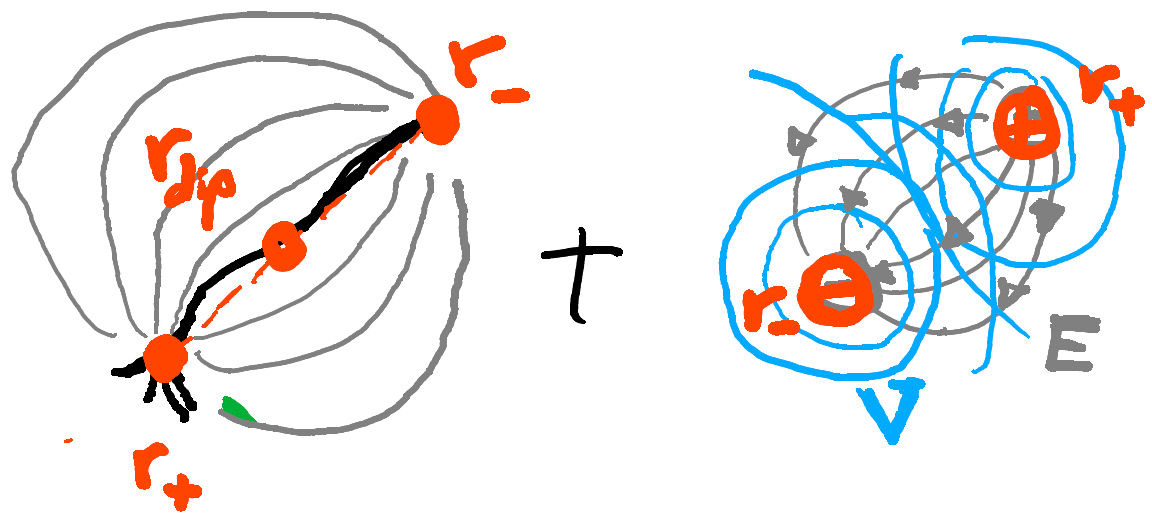
\includegraphics[width=0.4\linewidth]{./img_dev/nsNeuronDipole}
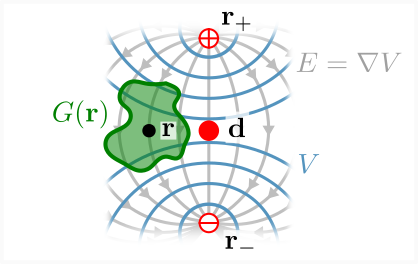
\includegraphics{./img_dev/CurrDensFieldOld}
\caption{Visual representation of a single dipole with electric sink and source located at $\dd^-$ and $\dd^+$, respectively.
%
We consider the position of the dipole, $\dd$, at the midpoint of $\dd^-$ and $\dd^+$.
%
The electrical field, $E= -\nabla V$, is shown as the lines of the fastest descent.
%
The divergence of $K = \nabla\cdot\ppar{\sigma E}$ is calculated as the limit of the surface integral of $K$ over $G(\rr)\rightarrow \sset{\rr}$, and it vanishes everywhere except at $\dd^+$ AND $\dd^-$.
%
In the quasi-static case, we assume that the magnetic field is constant in time, and thus, the time-varying influence over the electric fields is negligible}
\label{fig:diagrams1}
\end{figure}

With equations \eqref{eq:model1} and \eqref{eq:model2} at hand, we may determine the electric scalar field, $V$, in terms of the only dipole as
\begin{equation}
\nabla \cdot\ppar{\sigma(\rr)\, \nabla V(\rr) } = 
{\delta\ppar{\rr-\dd^+} - \delta\ppar{\rr-\dd^-}}
\label{eq:poisson_gral}
\end{equation}
or, in the isotropic case, as
\begin{equation}
\kappa \Delta V(r) = 
{\delta\ppar{\rr-\dd^+} - \delta\ppar{\rr-\dd^-}}
\label{eq:poisson_isotropic}
\end{equation}

It is relevant to recall that the EEG measurement from the only sensor is $V(\sa)$, with $\sa$ the locations of the EEG sensors.

%%%%%%%%%%%%%%%%%%%%%%%%%%%%%%%%%%%%%%%%%%%%%%%%%%%%%%%%
%%%%%%%%%%%%%%%%%%%%%%%%%%%%%%%%%%%%%%%%%%%%%%%%%%%%%%%%

\subsection{Boundary conditions Poisson equation}

To have a meaningful solution for equation \eqref{eq:poisson_gral} or \eqref{eq:poisson_isotropic} in the context of EEG, we must consider appropriate domain and boundary conditions.

Since the electric conductivity of air is very small compared with that of head tissues, it is straightforward to use the subject's head as a domain with reflective boundary conditions. 
%
Thus, the head is divided into a series of nested volumes, determined by both the biological tissues in place and their respective electric properties.

Under these conditions, the simplest model considers a small number of tissue-based regions as homogeneous isotropic media with constant conductivity; different media may have different conductivity.
%
The 4-sphere model considers only four media: the brain, $\mathcal{M}_4$, cerebrospinal fluid (CSF), $\mathcal{M}_3$, skull, $\mathcal{M}_2$, and the rest of the head, $\mathcal{M}_1$.
%
For computational purposes, we may consider a fifth medium, $\mathcal{M}_0$, representing the outside of the head.

Multiple approximations are used in practice, as illustrated in figure \ref{fig:diagrams2} where portions of the skull far from the brain are ignored, as well as muscle and connective tissues 
because those tissues are too far from the EEG sensors to make a significant difference in the model.

\begin{figure}
\centering
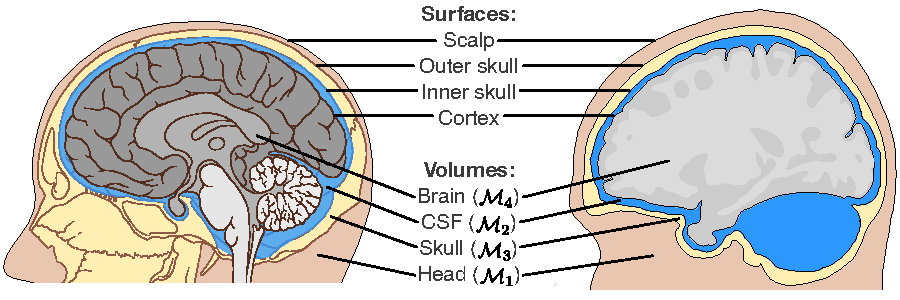
\includegraphics[width=\linewidth]{./img/HeadSurfacesVolumes}
\caption{Geometric domain defined by relevant tissues in the subject's head. The 4-sphere model considers three media: brain, cerebrospinal fluid (CSF), and the rest of the head. Relevant interfaces between media are displayed: brain cortex, inner and outer skull, and scalp. Notice the anatomical simplifications described in the text. (Left) Realistic illustration of a human head. Composition from two diagrams by Patrick L. Lynch and C. Carl Jaffe \cite{wikipic1, wikipic2}.  (Right) Cross-section of the surfaces obtained from the ICBM152 template after segmentation}
\label{fig:diagrams2}
\end{figure}

With the media defined formally, we may state the reflective boundary conditions,
\begin{equation}
\sigma(\rr)\, \nabla V(\rr) \cdot \mathbf{n} = 0, 
\text{ for } \rr \in \mathcal{M}_1
\label{eq:boundary1}
\end{equation}
where $\mathbf{n}$ is a vector orthogonal to $\partial\mathcal{M}_1$.
%
At the interfaces between media, the boundary conditions are to have continuous first derivatives; this property can be requested for the whole domain,
\begin{equation}
    V \in C^1\ppar{\mathcal{M}_1 \cup \mathcal{M}_2 \cup \mathcal{M}_3 \cup \mathcal{M}_4 }
\end{equation}

\subsubsection{Practical considerations}

Either equation \eqref{eq:poisson_gral} or \eqref{eq:poisson_isotropic} must be solved within the geometric regions described previously, subject to the boundary conditions in \eqref{eq:boundary1}.
%
The construction and treatment of those regions and the solution per se require special discussion.

Regions are often defined from the subject's anatomical data or an appropriately matched template.
%
The anatomical information is usually a T1 or T2 MRI, which is later segmented to identify relevant tissues. The segmented MRI is then used to obtain triangulated surfaces. 
%
More media can be incorporated into the model, such as a division of the brain into white matter and grey matter;
Those approaches are limited in the reliability with which these tissues can be identified.

Multiple commercial software is available for the segmentation of MRI and extraction of triangulated surfaces, such as ...

Once the triangulated surfaces are obtained, the equation can be solved numerically by either using Boundary Element Method (BEM), Finite Element Method (FEM), or others.

\subsection{Construction of the leadfield operator}

Recall that both equations \eqref{eq:poisson_gral} and \eqref{eq:poisson_isotropic} are constructed for one sensor and one dipole with unit magnitude.
%
We now consider a finite number of EEG sensors at locations $\sa_1, \sa_2, \dots, \sa_M \in \R^3$, and dipoles at locations $\dd_1, \dd_2, \dots, \dd_N \in \R^3$
with momenta $\mm_1, \mm_2, \dots, \mm_N$.
%
For ease of notation, write each momentum as
\begin{equation}
    \mm_n = \rho_n\, \ee_n
\end{equation}
with $\rho_n\in \R, \ee_n\in \R^3$ such that $\ee_n$ has unit norm, i.e. $\nnorm{\ee_n}_2 = 1$.

%
After making the assumptions described in the previous sections, we may conclude that the electric scalar field, $V$, is given by
\begin{equation}
V(\rr) = 
\sum_{n=1}^N \rho_n \tilde{V}_{n}(\rr)
\end{equation}
where $\tilde{V}_n$ is the solution to the following equation
\begin{equation}
\nabla \cdot\ppar{\sigma(\rr)\, \nabla \tilde{V}_n(\rr) } = 
{\delta\ppar{\rr-\dd_n^+} - \delta\ppar{\rr-\dd_n^-}}
\end{equation}
under the boundary conditions from equation \eqref{eq:boundary1}, and with each $\dd_n^\pm$ constructed from $\dd_n$.
%
For ease of notation, define 
\begin{align}
g(\rr, \dd_n) &= \tilde{V}_n(\rr)
\end{align}
and thus, we can write
\begin{equation}
V(\rr) = 
\sum_{n=1}^N \rho_n\, g\ppar{\rr, \dd_n} = 
\begin{bmatrix}
    g\ppar{\rr, \dd_1} & 
    g\ppar{\rr, \dd_2} &
    \cdots &
    g\ppar{\rr, \dd_N}
\end{bmatrix}
\begin{bmatrix}
    \rho_1 \\ \rho_2 \\ \vdots \\ \rho_N
\end{bmatrix}
\label{eq:back1}
\end{equation}
%\begin{equation}
%V(\rr) = 
%\sum_{n=1}^N \rho_n g\ppar{\rr, \dd_n} = 
%\spar{g\ppar{\rr, \dd_1}, g\ppar{\rr, d_2}, \cdots, g\ppar{r, d_N}}
%\spar{m_1, m_2, \cdots, m_N}\trans
%\label{eq:back1}
%\end{equation}

Furthermore, by using the equation for all the sensor locations and stacking the results, we obtain the following vector equation
\begin{equation}
\begin{bmatrix}
V\ppar{\sa_1} \\
V\ppar{\sa_2} \\
\vdots \\
V\ppar{\sa_M}
\end{bmatrix}
=
\begin{bmatrix}
    g\ppar{\sa_1, \dd_1} & 
    g\ppar{\sa_1, \dd_2} &
    \cdots &
    g\ppar{\sa_1, \dd_N} 
    \\
    g\ppar{\sa_2, \dd_1} & 
    g\ppar{\sa_2, \dd_2} &
    \cdots &
    g\ppar{\sa_2, \dd_N} 
    \\
    \vdots & \vdots & \ddots & \vdots
    \\
    g\ppar{\sa_M, \dd_1} & 
    g\ppar{\sa_M, \dd_2} &
    \cdots &
    g\ppar{\sa_M, \dd_N}
\end{bmatrix}
\begin{bmatrix}
    \rho_1 \\ \rho_2 \\ \vdots \\ \rho_N
\end{bmatrix}
\label{eq:model3}
\end{equation}

Equation \eqref{eq:model3} can be rewritten as the following generic matrix equation
\begin{equation}
\Y = \G\, \SA
\label{eq:model4}
\end{equation}
where $\Y \in \R^{M\times 1}$ encodes the EEG measurements, $\SA \in \R^{N\times 1}$ encodes the dipoles' magnitude, and $\G \in \R^{M\times N}$ is a matrix known as the leadfield matrix, gain matrix, forward operator, among other names; $\G$ encodes the mixture of current density to form the scalar electrical field measured by EEG sensors.

The forward model can be extended trivially to account for $T$ EEG measurements in time by setting $\Y \in \R^{M\times T}$, $\Y \in \R^{M\times T}$, and $\G$ unchanged; the resulting matrix equation will be identical to \eqref{eq:model4}.


If the dipole's orientation, $\ee_n$, is to be determined, we can consider each dipole as the sum of three dipoles parallel to some orthogonal directions. Such as in figure \ref{fig:diagrams3}, we can write
\begin{equation}
\rho_n \ee_n = \rho^x_n \ee_n^x + \rho_n^y \ee_n^y + \rho_n^z \ee_n^z
\end{equation}
with $\ee_n^x, \ee_n^y, \ee_n^z \in \R^3$ vectors with unit norm located at $\dd_n$ and parallel to the respective $x-, y-, z-$axis.
%

Under these new circumstances, equation \eqref{eq:back1} changes to
\begin{equation}
V(\rr) = 
\sum_{n=1}^N 
\spar{
\rho_n^x\, g\ppar{\rr, \ee_n^x} +
\rho_n^y\, g\ppar{\rr, \ee_n^y} +
\rho_n^y\, g\ppar{\rr, \ee_n^z}
}
\end{equation}
which can be written as a matrix equation such as \eqref{eq:model4}.

The overall effect of assuming unknown orientations are (1) the increase of the number of dipole magnitudes to be determined by a factor of 3, as well as the size of the leadfield matrix, and (2)
we need to compute the magnitude of these dipoles in order to recover the original interpretation.

\begin{figure}
\centering
%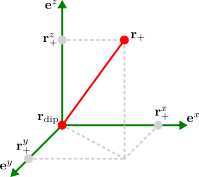
\includegraphics[width=0.4\linewidth]{./img_dev/OrthDecompOld}
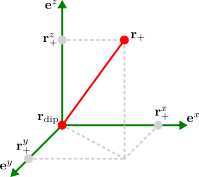
\includegraphics{./img_dev/OrthDecompOld}
\caption{Decomposition of an arbitrary dipole as a sum of projections into the three canonical directions.}
\label{fig:diagrams3}
\end{figure}

\section{Limitations of surface electrodes}



There are several neural activity patterns that surface electrodes cannot represent properly.
%
Silent activity refers to neural activity that doesn't produce a significant electric potential and is not registered by surface electrodes.
%
It is estimated that only 20\% of the brain's energy is spent producing non-silent activity.

The orientation of neuron dendrites, which carry the post-synaptic potentials, is crucial in how much of their activity is actually recorded by surface electrodes.
%
Pyramidal neurons at the gray matter (located at the outer cortex) are almost exclusively oriented parallel to the cortex surface.
%
This common orientation, combined with their physical proximity to the scalp, makes the pyramidal neurons to be over-represented on recordings from surface electrodes.

On the other side, neural activity occurring at the lower layers of the brain is more difficult to register and reconstruct.

These limitations of this recording modality are inherited from the ESI methods, and thus, they must be considered when interpreting the obtained results.

A second set of limitations from the distributed dipole model represents a spatial average of the .
%
Distributed dipoles can efficiently represent synchronous activity over large regions, a phenomenon known as a source patch.
%
Distributed dipoles of low magnitude may represent smaller source patches and regions with asynchronous orientations, resulting in .




%
The distributed dipole model is agnostic in that it doesn't make any assumptions about the location of the dipoles.
%
A region with no active dipoles leads to equivalent dipoles with zero magnitude, while a region with active dipoles leads to equivalent dipoles with non-zero magnitude.

\section{Extensions of the model}

The 4-sphere model is a prevalent standard in the modern literature.
%
Segmentation algorithms for the relevant tissues are available in many commercial software.

Different authors have addressed a number of limitations of the 4-sphere model.

For instance, extending the 4-sphere model into 5 spheres has been proposed by distinguishing between white matter and gray matter inside the brain.
%
The resulting model is almost identical, and the additional computational cost is not very large. 
%
%Unfortunately, 
However, the gray and white matter are very similar when observed using T1 MRI, even under normal conditions, and thus, very robust segmentation algorithms are required.

The assumption of isotropic conductivity has also been questioned.
%
Conductivity can be estimated using, for example, Diffusion Tensor Imaging.
%
[] investigated the benefits of including such additional information and concluded that anisotropic information should be used when available, but the enhancements do not justify the additional costs.

On the other hand, more simplistic models have also been proposed.
%
The Corrected 4-sphere model, for example, uses four spheres instead of volumes obtained from the subject.
%
TODO[ add comment]

Now, the 4-sphere model can be generalized to other types of electrical recordings.
%
For example, [] have used () to model intracranial electrodes, i.e., electrodes placed at the cortex surface or inside the brain.

In Chapter 3 we use the 1-sphere model to locate sources. 
\input literature.tex  % file containing Chapter 2 contents
\input model.tex       % file containing Chapter 3 contents
%\input virt_elec.tex      % file containing Chapter 4 contents
%%%%%%%%%%%%%%%%%%%%%%%%%%%%%%%%%%%%%%%%%%%%%%%%%%%%%%%%%%%%%%%%%%%%%%%%%%%%%%%%%%
%%%%%%%%%%%%%%%%                  Appendices                  %%%%%%%%%%%%%%%%%%%%
%%%%%%%%%%%%%%%%%%%%%%%%%%%%%%%%%%%%%%%%%%%%%%%%%%%%%%%%%%%%%%%%%%%%%%%%%%%%%%%%%%
%\appendix
%      \chapter{FIRST APPENDIX NAME}
%\chapter{INEQUALITY}
%\input appA.tex       % file with Appendix A contents
%\chapter{UPPER BOUNDS}
%\input appB.tex       % file with Appendix B contents
%%%%%%%%%%%%%%%%%%%%%%%%%%%%%%%%%%%%%%%%%%%%%%%%%%%%%%%%%%%%%%%%%%%%%%%%%%%%%%%%%%
%%%%%%%%%%%%%%%%                 Bibliography                 %%%%%%%%%%%%%%%%%%%%
%%%%%%%%%%%%%%%%%%%%%%%%%%%%%%%%%%%%%%%%%%%%%%%%%%%%%%%%%%%%%%%%%%%%%%%%%%%%%%%%%%

\bibliographystyle{abbrv} % We choose the "plain" reference style
\bibliography{./refs} % Entries are in the refs.bib file

%\renewcommand{\bibname}{REFERENCES}
%\bibliographystyle{plain}
%\nocite{*}      
%\input{mybib.tex}


%%%%%%%%%%%%%%%%%%%%%%%%%%%%%%%%%%%%%%%%%%%%%%%%%%%%%%%%%%%%%%%%%%%%%%%%%%%%%%%%%%
%%%%%%%%%%%%%%%%         Biographical Statement               %%%%%%%%%%%%%%%%%%%%
%%%%%%%%%%%%%%%%%%%%%%%%%%%%%%%%%%%%%%%%%%%%%%%%%%%%%%%%%%%%%%%%%%%%%%%%%%%%%%%%%%
\thebiography
\input biography.tex
\end{document}
